\subsubsection{UMD}

\textbf{UMD (UMIDADE-DO-SOLO):} A variável de saída UMD estabelece a referência de umidade que o solo deve possuir para o tipo de plantação em conjunto com todas as variáveis de entrada para um determinado momento da vida da planta (Germinação, Crescimento, Floração e Maturação).

\begin{figure}[h!]
\centering
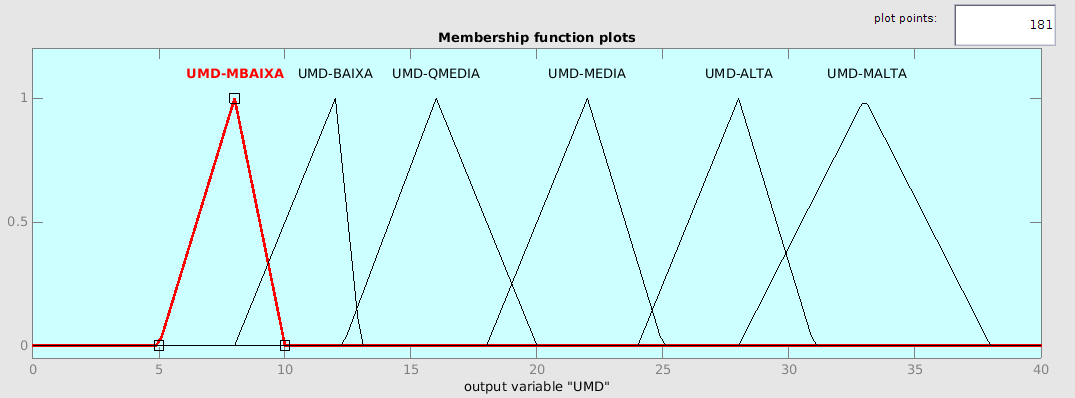
\includegraphics[width=1\linewidth]{Descricao/Imagens/UMD}
\caption{Umidade que se deseja para um determinado tipo de plantação}
\label{fig:UMD}
\end{figure}
